% CHANGERS LOG
% Dom 08/04 17:40 Dante
%  Melhorias menores no abstract (um pouco mais biito)
%  O que s�o "buscas constantes de informa��es"? � dito como se fosse algo concreto, mas eu achei confuso (l63)
%  Estocasticidade ou Estocacidade?
\documentclass[10pt, conference, compsocconf]{IEEEtran}

%Pacotes Gerais
\usepackage{mathtools}
\usepackage{float}
\usepackage{nameref}
\usepackage{graphicx,url}

\usepackage[latin1]{inputenc}
%\usepackage[portuges,brazilian]{babel}
\usepackage[english]{babel}
\usepackage[T1]{fontenc}

\hyphenation{op-tical net-works semi-conduc-tor}

\begin{document}

% >mateus: - ver se maintaining n�o fica melhor do que keeping
% >iuri: oras eu acho que sim, mas devemos tirar o the entao antes do Quality
\title{Cognitive Mesh Networks: Maintaining Transmission Quality Using Analysis and Prediction of Traffic with Artificial Neural Networks}

\author{\IEEEauthorblockN{Iuri Andreazza}
\IEEEauthorblockA{Unidade Acad�mica de Gradua��o\\
UNISINOS\\
S�o Leopoldo, Brazil\\
iuri.andreazza@gmail.com}
\and
\IEEEauthorblockN{Dante Moreira Zaupa}
\IEEEauthorblockA{Unidade Acad�mica de Gradua��o\\
UNISINOS\\
S�o Leopoldo, Brazil\\
dantezco@gmail.com}
\and
\IEEEauthorblockN{Mateus Raeder}
\IEEEauthorblockA{Unidade Acad�mica de Gradua��o\\
UNISINOS\\
S�o Leopoldo, Brazil\\
mraeder@unisinos.br}
}


\maketitle

\begin{abstract}
The need for greater quality of service demands more from the infrastructure of existing network models. Considering the growth rate of devices on the network requesting data constantly, these models will soon become obsolete due to their inability to provide constant access to the network without requiring the user to configure their devices each time the network changes. Mesh Network model provides constant access to the wide network, but it has several problems, such as the difficulty of maintaining the quality of services by providing links with speed and performance desired. In this paper we propose a new approach to package routing in the mesh model, in order to combine the flexibility of Artificial Neural Networks, aiming at maintaining network performance in the face of changing topology.

\end{abstract}

\begin{IEEEkeywords}
Mesh Networks; Artificial Neural Networks; Routing Algorithms; Cognitive Routing;

\end{IEEEkeywords}

\IEEEpeerreviewmaketitle

\section{Introduction}\label{sec:intro}

%seguindo o modelo do RA - A introdu��o j� est� boa e tamb�m cont�m um intro das redes mesh e redes neurais

At the end of the 20th century and beginning of the 21st century, the evolution of computing and communication technologies made mobile computing and wireless computer networks widespread, which increased their presences in academic, industrial and home environments. This allows anyone to easily access computer networks and databases information. The main issue that stress wireless networks is the increasing presence of notebooks, cell phones and many other mobile devices that enjoy the infrastructure to access the Internet. With the availability of online services and tools for both desktop and mobile devices users, the need for constant information and connectivity becomes essential, as well as the quality of that information \cite{Zhu:1276870}.

Data networks clients are more and more present in the digital world and they demand constant connectivity. With the advent of online and digital tools, the need for quality of connection rises, forcing the current infrastructure to almost achieve its limit. Although networks can support a great amount of users with high level of quality, these models did not predict new incoming users (common day-do-day devices) like refrigerators, cell phones, tablets, printers, information center, cars and houses, for example. The omnipresence of computational devices stresses the network structure, since it foresees that the whole environment will be connected to the devices, thus needing a constant and intense data flow \cite{Akyildiz:1509968}\cite{Zhu:1276870}.

%Introducao MESH

Most common wireless networks works in a centralized way, \textit{i.e.}, there is a single access point for all clients. In these scenarios, the network becomes exposed to failures and if the access point becomes unavailable or unreachable, all of its clients lose the network connection. An existing pattern that provides a scenario in which even if the access point is down the connection among the clients still exists, is the mesh pattern. This model of network has some important functionalities such as self-repairing, self-configuration and self-layout (among others), giving an advantage over other models \cite{Akyildiz:1509968}.
However, the mesh model currently does not offer a good support for quality of service, \textit{i.e.}, data transmission inside the mesh is slow and tends to need retransmission, making it impractical to maintain a constant stream of data to the clients in the mesh.

With these new types of users joining the mesh infrastructure out of research environments, this model becomes interesting for a large scale implementation. In this way, it is possible to make an environment in which new devices can join the existing ones. This situation will naturally create a ``computational ecosystem'' of devices, besides reducing the need for users to manually configure each device.

However, this growth of users inside the mesh creates a totally stochastic environment, which generates a great loss of quality in the routing process algorithms (in the maintenance of the data flow). This problem is a main factor for the resistance against large scale adoption of the mesh model, not allowing users to take advantage of its capabilities.

%Introdu��o RNA

In the constant search for more flexible mechanisms, capable of adapting to the constant changes in topology (that are natural in a mesh network), we propose the use of Artificial Neural Networks (ANNs) to improve the mesh model packet routing process. ANNs have the ability for non-linear and parallel processing, which gives the capacity to process and classify data in a cognitive way with high efficiency. 

To make them efficient, it is necessary to train the ANNs with a base set of scenarios and its expected results. This learning process is called ``supervised training'' and has as objective to prepare the internal structures with values (weights) of the ANNs to respond with the expected values whenever they find a known pattern \cite{Claudio:1996}.

ANNs are built like parallel distributed systems, composed by small simple processing units: the artificial neurons. These neurons calculate mathematical functions, which are usually non-linear functions, and are organized in layers. Artificial neurons are interconnected by a large number of connections, which are usually unidirectional (see Figure~\ref{fig:rna_visao_classica}). There are still different models that use backpropagation connections, for example \cite{Simon:2001}.
% >Dante: pra mim, essa �ltima frase ficou meio solta.

\begin{figure}[h]
	\centering
	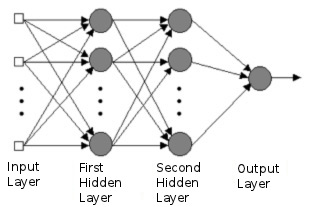
\includegraphics[width=0.4\textwidth]{./graphics/rna_visao_classica_hopfield_en.jpg}
    \caption{ Classic visualization of the structure of a neuron in an Artificial Neural Network \cite{Braga:2007}.}
    \label{fig:rna_visao_classica}
\end{figure}

\section{Mesh Networks Routing Problems}\label{sec:routing}

Mesh network ecosystem brings up a problem related to the dataflow among the different devices and the Internet, impacting directly on connection quality. Considering that a device requires a constant data stream, the network has to be able to maintain the flow of data, always selecting the shortest cost path \cite{Baransel:386051}. Given this problem, maintain efficiency in the network becomes a vital issue. In this context, the development of new technologies is expected to allow the mesh model to have the necessary flexibility, in order to hold large scale applications.

The self-organization and self-repairing capabilities are great characteristics of the mesh model. They make the network to be flexible, and almost fail-safe. However, these characteristics impose a great computational cost for the decision process in the retransmission and routing of packets. These problems represent how stochastic is the network topology: with the constant changes in the topology (the entry and exit of client nodes and possible failures in mesh routers) the network unfit for algorithms that converge to static models, that do not adapt to change.

Trivial algorithms are not capable of adjusting themselves in time to support the changes in the network \cite{Baumann:4390832} \cite{Zhi:5364647} \cite{Song:5072224}. The authors of \cite{Baumann:4390832} present the traditional AODV (Ad Hoc On Demand Distance Vector) and its inability to supply a quality routing for the model. As an enhancement, these same authors demonstrate a version of the AODV-GW (which is specialized for mesh networks) as an alternative, and they compare it to other protocols, one of those proposed by themselves: FBR, the Field Beacon Routing.

FBR proposes a proactive alternative to routing, making the client nodes to inspect their environment searching for their neighbours, thus ``seeing'' the whole ecosystem around and using it in its favour in the decision process of packet routing.

\begin{figure}[h]
	\centering
	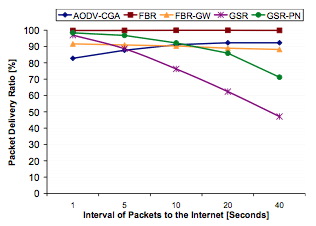
\includegraphics[width=0.4\textwidth]{./graphics/Baumann_1.png}
    \caption{ Average packet delivery of packets in a scenario containing pedestrians connected to the ecosystem. \cite{Baumann:4390832}.}
    \label{fig:Baumann_1}
\end{figure}

\begin{figure}[h]
	\centering
	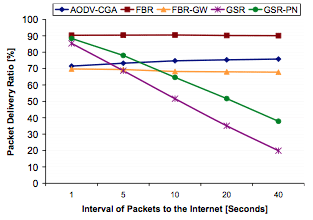
\includegraphics[width=0.4\textwidth]{./graphics/Baumann_3.png}
    \caption{ Average packet delivery in a scenario consisting of cars connected to the ecosystem. \cite{Baumann:4390832}.}
    \label{fig:Baumann_3}
\end{figure}

After analysing the graphics (Figures~\ref{fig:Baumann_1},~\ref{fig:Baumann_3} and~\ref{fig:Baumann_2}) presented by the author, in \cite{Baumann:4390832}, it can be concluded that, the bigger the mobility of client nodes the higher the interruptions in packet delivery. Thus, package delivery becomes compromised and the throughput drops. Consequently, the end user of the ecosystem will see a significant drop in network performance.

\begin{figure}[h]
	\centering
	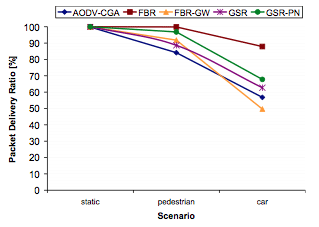
\includegraphics[width=0.4\textwidth]{./graphics/Baumann_2.png}
    \caption{ Average packet delivery in a scenario containing static client nodes. \cite{Baumann:4390832}.}
    \label{fig:Baumann_2}
\end{figure}

The analysis of Figure~\ref{fig:Baumann_2} shows that scenarios where the client nodes are static, package routing tends to work correctly, even with classic protocols. However, it is also possible to notice that, in scenarios where client nodes are mobile and have random behaviour, package delivery becomes effectively lower.

\section{Cognitive Routing with Neural Networks}\label{sec:neural_mesh}

In our work, neural networks are used in the routing protocol of the mesh network. More specifically in the packet retransmission process, like in the works presented by other authors \cite{Venkataram:2002:NNB:638963.638974}, which focus their efforts in the search for better paths using traffic analysis and prediction. This work, on the other hand, focuses in the process of decision during retransmission of a packet. The protocol will use the neural network to decide what is the best path for a packet to follow, routing it to less loaded paths, in order to avoid path overloading.

The main idea of cognitive routing is to provide the flexibility that devices participating in the mesh need to use efficiently the available resources. The use of Artificial Neural Networks in the package routing becomes significant in the performance of the mesh because it provides flexibility and agility in the distribution of information through the topology. The employment of traffic engineering in the information flow over the network is extremely important, since the network topology stochasticity imposes great challenges in connection quality. With that in mind, congnitivity appears to allow the network to be flexible enough, foreseeing its future stages, and maintaining quality at an acceptable level \cite{Venkataram:2002:NNB:638963.638974}\cite{Zhi:5364647}\cite{Song:5072224}.

%OLD
%The Hybrid Wireless Mesh Protocol, or HWMP, works in a proactive and reactive way, combining, in an on-demand fashion, the discovery of paths and the construction of a routing table. Because of this strategy, the protocol enables the client nodes to communicate themselves in a peer-to-peer way. This protocol is used in client nodes that inhabit frequently changing environments. The basic routing metric used in this protocol is the resource of the transmission channel of a given link~\cite{IEEE:8011:11s}.

The Hybrid Wireless Mesh Protocol (HWMP) works pro-active and reactive, combining on demand the path discovery and the routing table building. Because of that the strategy, the protocol allows the client nodes to communicate in a peer-to-peer way. This protocol is used for client nodes that are in environments with great and constant changes. The basic routing metric used in this protocol shall be the resource consumption of the transmission channel for a particular link~\cite{IEEE:8011:2s}.

%OLD
%The process of cognitive routing has, as base of execution, the HWMP protocol, which was changed so that, during the packet broadcast process, that is, before the next jump of the package, it runs the ANN instantiated for that client node and evaluates the target node. This evaluation determines if the packet will do the jump to the target, or if the protocol should choose another node.

The cognitive routing process in our work is based on the HWMP protocol. This protocol has been adjusted for partially support the use of the ANN during the broadcast of a package: before the next hop of the package, the ANN is performed in order to evaluate and instantiate the target node of the jump. This evaluation determines whether the package will make the jump to the same node or whether the protocol should choose another node to jump.

\subsection {ANN Structure}

The ANN used was a Hopfield network with two inputs, one output and three neurons in the hidden layer. During the simulation process, this default setting of the ANN proved to be viable and stable, reaching the threshold that allowed for speed and stability in changing scenarios, \textit{i.e.} mobile client nodes. The ANN uses the sigmoid function to operate using the backpropagation to adjust the network weights. The parameters used to run the network as follows:

\begin{itemize}\label{lst:1}
	\item Number of Inputs: two;
	\item Number of outputs: one;
	\item Number of Hidden Layers: tree;
	\item Number of Layers: tree;
	\item Desired Error: 0.0001;
	\item Max Epochs: 1000;
\end{itemize}

The parameters used were stable during the construction of the training sets as well as at the time that the network runs for evaluating the data of the destination nodes. Although the construction naive the results obtained by stable ANN are good and worth of further investigation.


\subsection{Mesh Routing Metrics}

The metrics currently used in the assessment of the target mesh are the Delay and the Packet Forwarding PDF (Packet Delivery Fraction). These metrics can determine how much the client node is overloaded, both forwarding packets or other processes taking context and occupying the processing time. With these starting geometries, initial data has been compiled (Table~\ref{tab:base}) with the output patterns.

\begin{table}[h]
	\begin{center}
	\begin{tabular}{|l|l|}
		\hline
		PDF (Packet Delivery Fraction) 	& Avg. Delay \\ \hline\hline
		91.20\%	& 0.015578 \\ \hline
		85.57\%	& 0.0179017 \\ \hline
		98.23\%	& 0.00939786 \\ \hline
		99.55\%	& 0.00592165 \\ \hline
		91.74\%	& 0.015798 \\ \hline
		61.54\%	& 0.0734161 \\ \hline
		65.60\%	& 0.18154 \\ \hline
		67.48\%	& 0.0329183 \\ \hline
		79.58\%	& 0.0166734 \\ \hline
		70.57\%	& 0.0323162 \\ \hline
	\end{tabular}
	\caption{Sample database collected for the training scenarios of the network.}
	\label{tab:base}
	\end{center}
\end{table}

%OLD
%The threshold for determining whether a node is overloaded was set at seventy percent of the PDF. That shows that there is a low rate of delivery of packets, while also showing that it has a high delay in deliveries. These data inform the client node is failing to forward packets successfully.

The threshold for determining whether a node is overloaded was set on seventy percent of PDF, where it can be seen that there is a low package delivery index, at the same time can be seen that it has high delay deliveries. Such data will inform the client node that it is not able to forward the packets.

\subsection{ANN Training and Execution}

% >Dante: And here I stopped

%The training of the neural network happens disconnected from the simulation. So having these scenarios being generated through analyzes of patterns starting prior to routing simulation. Such scenarios indicate cases where the network have the positive output and indicate that the client node of the target jump is within the range to maintain the nominal data stream.

Neural network training is done in a disconnected state from the simulation. So the scenarios are being generated prior to the reviews from routing simulation patterns. Such scenarios indicate the cases in which the network should have its positive output indicating that the client node package jump target is within the parameters considered nominal maintenance of data flow.

%The implementation of ANN occurs in the process of packet retransmission, at each relay the packet's destination is evaluated by the ANN, which determines (according to the training scenarios) if the destination node isn't overloaded.

The implementation of ANN occurs within the process of packet relay, each retransmission the destination of the packet is evaluated by the ANN, which determines (based training scenarios) if the node is overloaded or not.

Such information about the client neighbouring nodes is obtained in the MACAddress that is changed to also transmit their data in PDF and Delay. In order to take the proactive and reactive nature of the network, the neighbours in each update the data is also updated. So the ANN is able to evaluate the destination node and determine whether or not that packet should be used in the forwarded route.

\section{Simulation Results}

% >Dante: "estruturas fara�nicas"?
To generate and evaluate the results we simulate a mesh network with some characteristics using the NS-3, a simulator based on discrete events for the community of researchers and educators. This simulator aims at providing an environment for the study of large-scale networks (for example, the Internet and huge structures), with controlled environments. NS-3 has the following features for running the simulations~\cite{NS3:1}.

\begin{itemize}
	\item Is written in C++ with an optional interface for Python;
	\item Provides integration with software that follow their patterns of arrival and departure information, enabling other tools to be used in conjunction with the simulator;
	\item The research, in general, is validated in two ways: through simulations and real implementations. The NS-3 is an organization that resembles the physical implementations, thus allowing to test more accurately the simulations;
	\item Contains codes that allow integration with the Linux kernel modules allowing the simulator operates in conjunction with real data. As their model is relatively close to the actual implementation, it supports device drivers as well as IP and Sockets APIs (Linux);
	% >Dante: q?
	\item Eases test simulating in real environments, as well as real time experiments;
	\item Contains a rich documentation on the operation of their strata and classes, stating what each part of the code available in the simulator does;
	\item Its new reporting model is compatible with external tools, such as Wireshark.
\end{itemize}

%An example scenario is designed to be configurable and can therefore be changed to generate alternative outcomes for comparative basis. The parameters of the base scenario are:

An example scenario were designed to be configurable, so it can be changed to generate alternative results for comparative basis. The base scenario parameters are:

\begin{itemize}
	\item \emph{x-size}: Width of the grid, default 6;
	\item \emph{y-size}: Height of grid, default 6;
	\item \emph{step}: Space on the grid edge, default 100m; 
	\item \emph{step}: Time from randomization to the start of transmission of packets (0.1 second);
	\item \emph{time}: Simulation time, default 100 seconds;
	\item \emph{packet-interval}: Transmission interval of the packets, default 0.001 second;
	\item \emph{packet-size}: Packet Size, default 1024bytes;
	\item \emph{interfaces}: Number of transmission interfaces (antennas) that possess a client node, default 1;
	\item \emph{channels}: Number of transmission channels for a client node, default 1;
	\item \emph{pcap}: Enable PCAP to generate trace files, default true;
	\item \emph{stack}: Model of the network stack used, default \emph{ns3::Dot11sStack};
	\item \emph{root}: MAC address of the base node of the grid.
\end{itemize}

The graphs presented serve as a basis for evaluating the use of neural networks in the decision process of the packet routing within the mesh. The graph in Figure~\ref{fig:g1} shows the average delivery of packets from a data stream, also the average rate of transmission. The relay presented shows which packages have been retransmitted before arriving at the destination.

\begin{figure}[h]
	\centering
	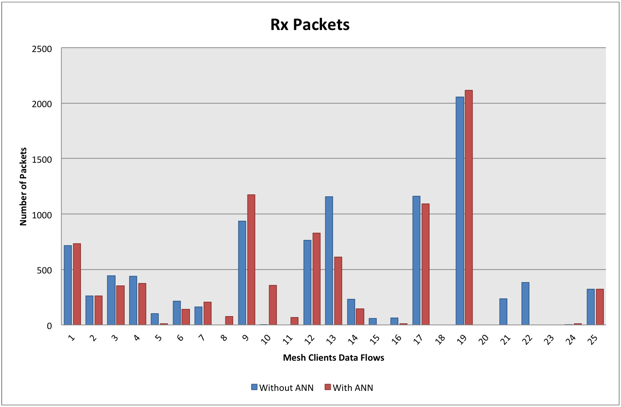
\includegraphics[width=0.5\textwidth]{./graphics/image007.png}
    \caption{ Average delay and packet delivery rate Transmission and Retransmission.}
    \label{fig:g1}
\end{figure}

% >iuri: Apresentar o gr�fico do throughput da rede

%A Figura~\ref{fig:g8} apresenta a m�dia de atraso nas entregas de pacotes em cada fluxo de dados.

%\begin{figure}[h]
%	\centering
%	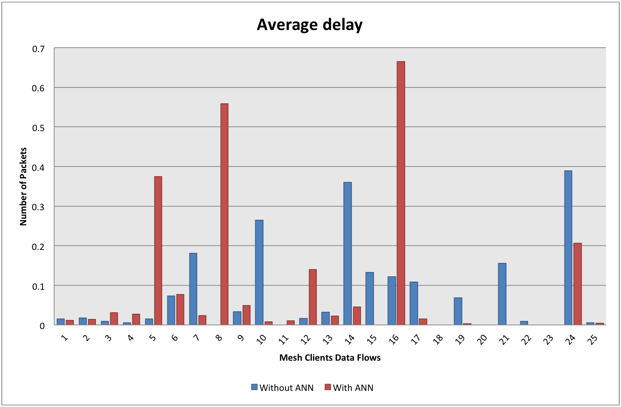
\includegraphics[width=0.5\textwidth]{./graphics/image008.png}
%    \caption{ M�dia de entrega de pacotes.}
%    \label{fig:g8}
%\end{figure}

%\begin{figure}[h]
%	\centering
%	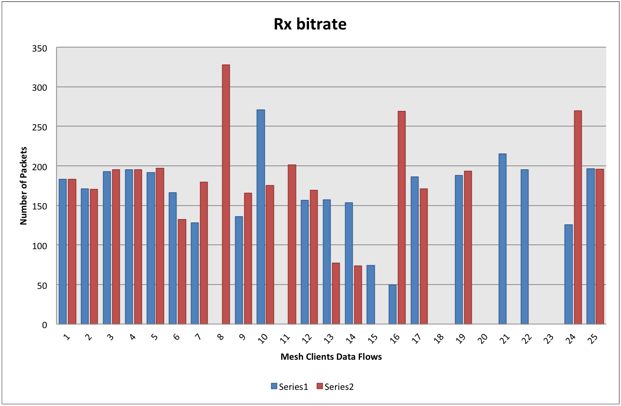
\includegraphics[width=0.5\textwidth]{./graphics/image009.png}
%    \caption{ Porcentagem de pacotes entregues.}
%    \label{fig:g9}
%\end{figure}

%\begin{figure}[h]
%	\centering
%	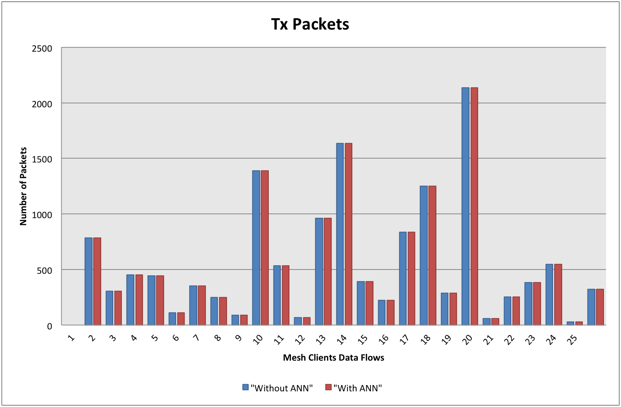
\includegraphics[width=0.5\textwidth]{./graphics/image010.png}
%    \caption{ Porcentagem de pacotes entregues.}
%    \label{fig:g10}
%\end{figure}

The PDF shown by the ANN varies in different simulations, as seen (Figure~\ref{fig:g11}) that each data stream in the PDF remains close to the standard network and at times managed to maintain a higher rate of packet delivery than the trivial algorithm.

\begin{figure}[h]
	\centering
	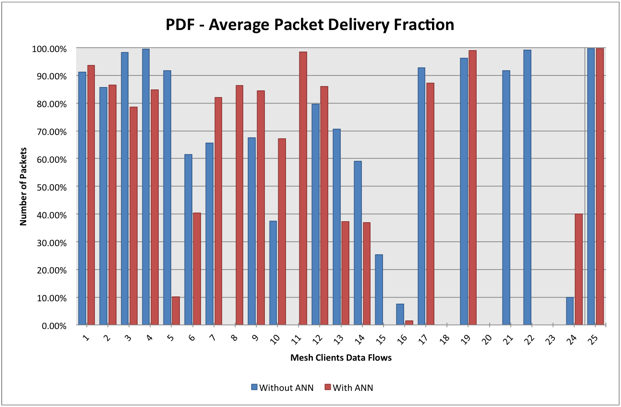
\includegraphics[width=0.5\textwidth]{./graphics/image011.png}
    \caption{ Average packet delivery fraction.}
    \label{fig:g11}
\end{figure}

It is possible to notice that in Figure~\ref{fig:g12} the ANN represents (in many cases) a much lower rate of packet loss, thus demonstrating that the decision to go for alternative paths may be feasible in cases of overload.

\begin{figure}[h]
	\centering
	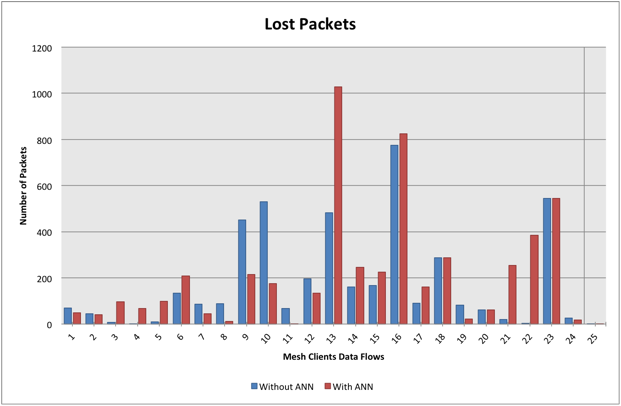
\includegraphics[width=0.5\textwidth]{./graphics/image012.png}
    \caption{ Lost Packets.}
    \label{fig:g12}
\end{figure}

\begin{figure}[h]
	\centering
	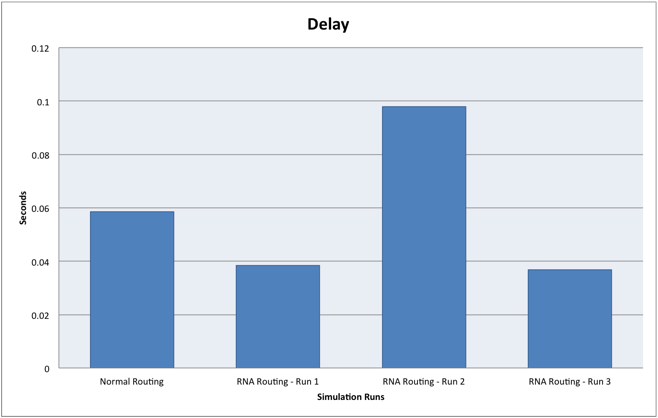
\includegraphics[width=0.5\textwidth]{./graphics/image013.png}
    \caption{ Delivery delay.}
    \label{fig:g13}
\end{figure}

Figure~\ref{fig:g13} compares three simulations using ANN and a simulation of the standard protocol, as well as (Figures~\ref{fig:g14}~\ref{fig:g15}) it is possible to note significant changes to the PDF and throughput. Seeing that the rate of delay of the simulations being evaluated as a whole tends to be lower, but because that packages spend more time jumping around so the throughput tends to be lower than the standard without using ANNs.

\begin{figure}[h]
	\centering
	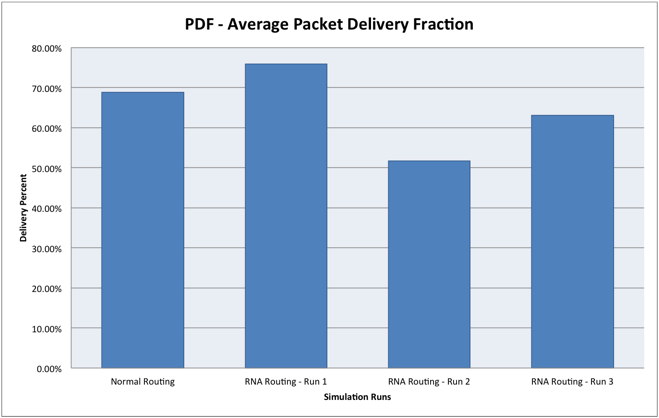
\includegraphics[width=0.5\textwidth]{./graphics/image014.png}
    \caption{ Percentage of packets delivered.}
    \label{fig:g14}
\end{figure}

\begin{figure}[h]
	\centering
	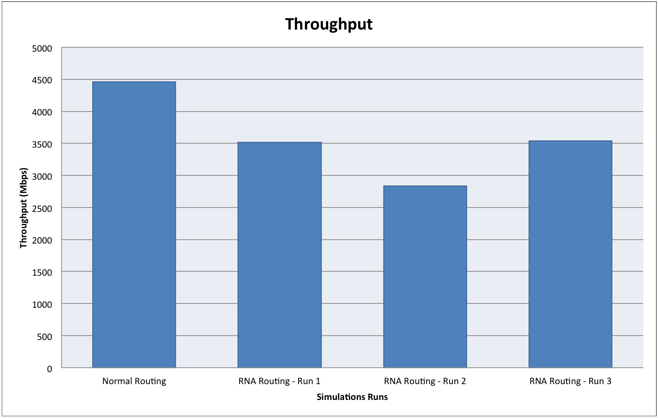
\includegraphics[width=0.5\textwidth]{./graphics/image015.png}
    \caption{ Average Packet lost.}
    \label{fig:g15}
\end{figure}



% >Dante: Rev� as �ltimas linhas aqui!
% >Iuri: ok, revisto... (falar sobre a quest�o do overhead dos dados ... normalizados).
The use of ANNs in the simulation adds a significant overhead so that the results presented appear to be worse than the trivial routing algorithms. However, it is considered a full-scale applicability and use of ANNs in hardware the probability that the results inherent in the simulation become much more attractive \cite{Akyildiz:2006:NGS:1162469.1162470}.


\section{Related Work}

Some authors have worked with models of ANNs to solve problems related to the mesh network and its basic structure. A major problem in this model is the optimal routing of packets, directly influenced by the chaotic structure that form mesh networks. One approach is found solving the optimal path routing in artificial neural networks~\cite{Venkataram:2002:NNB:638963.638974}.

%The authors of~\cite{Venkataram:2002:NNB:638963.638974} apply neural networks in order to solve the problem of finding the shortest path between a client node start and end a client node. The same study identified a real application for which ANN would be necessary to route the implementation of the hardware level, because the time required for adjustment of the network weights, and the convergence time in the software level is too expensive.

The authors of~\cite{Venkataram:2002:NNB:638963.638974} apply neural networks in order to solve the problem of finding the shortest path between clients, start and end. The same study identified a real application for which ANN would be necessary to route the implementation of the hardware level, because the time required for adjustment of the network weights, and the convergence time in the software level is too expensive.

Another paper that applies ANNs within the model of mesh networks is the work described in~\cite{Zhi:5364647}, which points out the challenges in the use of ANNs to achieve high levels of quality in mesh networks. In the paper, the authors present the modified ANNs to support the ability to measure the flow of information within the client-nodes, in order to create a mechanism for routing flexible enough to support the stochasticity of the network topology. This application is based on the ability of ANN from a mathematical analysis of a series to predict whether a future event on the client node will have its ability to relay packets compromised.

The work described in~\cite{Song:5072224} is a complete study of the behavior of users of infrastructure mesh networks that is being raised the issue of stochasticity of traffic from the random behavior of users. Given this premise, the paper proposes a fully distributed algorithm for routing, able to be flexible to accommodate changes in network infrastructure.

However, in this paper the idea is to use the ANNs fully operational in routing decision, as in~\cite{Zhi:5364647} and~\cite{Venkataram:2002:NNB:638963.638974} to use this cognitive mechanism to decide if the current path where the package is valid and if the next hop will not be compromised. If the path in the near future is not practicable, then forward the packet to another client node being more efficient compared to others available.

\section{Conclusion}\label{sec:con}

A point to get is the feasibility to simulate an ANN in each node; now the training is done so disconnected from the simulation process. Thus the training scenarios of the network were created prior to the simulation and only used the process of evaluating the neural network. As future implementation using a dynamically driven recurrent network is used. This model is able to function without the training cases, self-adjusting during the duration of the active node and thereby enabling each node to fit the environment where they are.

The simulations showed consistent results but require further study because in some cases there was a decline in the quality of the network. Such anomalies occur during the simulations because the current algorithm implemented only evaluates the next node that the package will be sent. This ANN does not assess the status of client nodes where being forward. However, in most cases even a client node being evaluated in the path data show promising results, causing the network circumvent stress conditions avoiding paths that become unstable. These good results are promising and require further study, leaving the network with higher connectivity and higher quality.

% use section* for acknowledgement
%\section*{Acknowledgment}

%Eu gostaria de agradecer pelas revis�es, Mateus e Dante assim como suas %contribui��es na escrita deste trabalho .... nao sei o que escrever nesta se��o.

%(pedir para o Felipe corrigir tamb�m? seria uma boa)

\bibliographystyle{./sbrn_iuri}
\bibliography{./sbrn_iuri_abrv.bib,./sbrn_iuri.bib}

%\begin{thebibliography}{1}

%\bibitem{IEEEhowto:kopka}
%H.~Kopka and P.~W. Daly, \emph{A Guide to \LaTeX}, 3rd~ed.\hskip 1em plus
%  0.5em minus 0.4em\relax Harlow, England: Addison-Wesley, 1999.

%\end{thebibliography}

\end{document}